\usepackage[authoryear,round]{natbib}

\newcommand{\sheetnum}{%
	07
}
%\setcounter{section}{\sheetnum-3}
\newcommand{\tutorialtitle}{%
    Recurrent neural networks
}
\newcommand{\tutorialtitleshort}{%
	RNNs
}
% for slides
\subtitle{\sheetnum \tutorialtitle}

\maxdeadcycles=1000 % Workaround for ! Output loop---100 consecutive dead cycles because of too many figures

% The following use of algroithms does not work well with the notes:
%
%
%
%
% instead use the following for your algorithms:
%
%\begin{figure}[!t]
%\removelatexerror
%\begin{algorithm}[H]
    % your algo here
    %\label{alg:algolabel}
    %\caption{algocaption}
%\end{algorithm}
%\end{figure}
%\begin{algorithm}
% Below is the definition for the command \removelatexerror:
\makeatletter
\newcommand{\removelatexerror}{\let\@latex@error\@gobble}
\makeatother

\begin{document} %%%%%%%%%%%%%%%%%%%%%%%%%%%%%%%%%%%%%%%%%%%%%%%%%%%%%%%

\sheet{\sheetnum}{\tutorialtitleshort}

\ttopic{\tutorialtitle}

\columnratio{0.2,0.8}\textbf{}
\begin{paracol}{2}
%\setlength{\columnseprule}{0.1pt}
%\setlength{\columnsep}{5em}

\begin{rightcolumn}

% notes version will ignore it
\begin{frame}
\titlepage
\end{frame}

\begin{frame}
\tableofcontents
\end{frame}

\mode<all>
\section{Recurrent Neural Networks (RNNs)}

\begin{frame}\frametitle{\subsecname}

\begin{itemize}
\item Feedforward networks:\\

\underline{Data}:
\begin{equation*}
\Big\{ \left(\vec x^{(\alpha)}, \vec y^{(\alpha)}_{\mathrm{True}} \right) \Big\}\,,\quad \alpha = 1,\ldots,p
\end{equation*}

\pause

\begin{itemize}
\item any two sample pairs $\left(\vec x^{(\alpha)}, \vec y^{(\alpha)}_{\mathrm{True}} \right)$ and $\left(\vec x^{(\alpha')}, \vec y^{(\alpha')}_{\mathrm{True}} \right)$ are assumed to be \iid
\item Their respective predictions $\vec y(\vec x^{(\alpha)}; \vec w)$ and $\vec y(\vec x^{(\alpha')}; \vec w)$ are also independent from one another.
\end{itemize}

\pause

\item RNN \corresponds~Neural network with loops.\\

\underline{Data}:\\

\begin{equation*}
\Big\{ \left(\vec x^{(\alpha,t)}, \vec y^{(\alpha,t)}_{\mathrm{True}} \right)_{t=1}^{n_{\alpha}} \Big\}\,,\quad \alpha = 1,\ldots,p
\end{equation*}

\pause

\begin{itemize}
\item $p$ \iid sequences
\item each sequence $\alpha$ contains $n_{\alpha}$ time steps
\item Use information from the previous step to predict the next step.
\end{itemize}

\end{itemize}

\end{frame}


\subsection{Basic RNN}

\mode<presentation>{

\begin{frame}\frametitle{\subsecname}

\begin{figure}[ht]
     \centering
	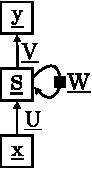
\includegraphics[width=0.2\textwidth]{img/rnn}
     \mode<article>{
	\caption{Basic RNN architecture}
	}
	\label{fig:rnn} 
\end{figure}
\end{frame}
}

\begin{frame}\frametitle{\subsecname}

%Omitting sequence index $\alpha$
\begin{figure}[ht]
     \centering
	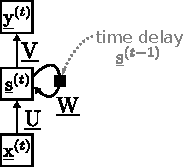
\includegraphics[width=0.4\textwidth]{img/rnn_time_delay}
     \mode<article>{
	\caption{Basic RNN architecture}
	}
	\label{fig:rnn_time_delay} 
\end{figure}


\end{frame}

\subsubsection{The tunable parameters of a basic RNN}

\definecolor{darkgreen}{rgb}{0,0.6,0}

\begin{frame}\frametitle{\subsubsecname}

\mode<article>{
\begin{figure}[ht]
     \centering
	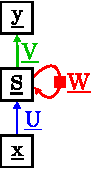
\includegraphics[width=0.2\textwidth]{img/rnn_colored}
     \mode<article>{
	\caption{Basic RNN architecture}
	}
	\label{fig:rnn} 
\end{figure}
}
\mode<presentation>{
\placeimage{13}{1}{img/rnn_colored}{width=2cm}
}

Let
\begin{itemize}
\item[] $N$ be the number of input variables $\rightarrow$ $\vec x^{(t)} \in \R^N$
\item[] $H$ be the number of hidden nodes
\item[] $M$ be the number of output nodes
\end{itemize}

\pause

Identify the free parameters (trainable weights) of the network:

\begin{itemize}
\item input-to-hidden: ${\color{blue} \vec U = (\vec u_1,\ldots, \vec u_i, \ldots,\vec u_H)} \in \R^{H,N}$
\item hidden-to-hidden: ${\color{red} \vec W = (\vec w_1,\ldots, \vec w_j, \ldots,\vec u_H)} \in \R^{H,H}$
\item hidden-to-output: ${\color{darkgreen} \vec V = (\vec v_1,\ldots, \vec v_k, \ldots,\vec v_H)} \in \R^{M,H}$
\end{itemize}




\end{frame}

\begin{frame}\frametitle{Weight matrices in basic RNN}
Remark: The weight matrices are constructed slightly differently than how we defined them for MLPs. We now stack row vectors instead of column vectors
Reason: brevity, to avoid putting transpose everywhere

\begin{itemize}
\only<1>{
\item input-to-hidden:\\

The weights from each input $x_j$ to each hidden node $h_i$:
\begin{equation}
\vec u_i = (\vec u_{i1},\ldots, \vec u_{ij}, \ldots,\vec u_{iN}) \text{ with } j=1,\ldots,N \text{ and } i=1,\ldots,H
\end{equation}

\begin{equation}
\vec U = 
\left(
\begin{array}{ccc}
  \horzbar & \vec u_1 &  \horzbar \\
  \horzbar & \vec u_2 &  \horzbar \\
		   & \vdots    &          \\
  \horzbar & \vec u_H &  \horzbar
\end{array}
\right) \in \R^{H,N}
\end{equation}
}
\only<2>{
\item hidden-to-hidden:\\

The weights to each hidden node $h_i$:
\begin{equation}
\vec w_i = (\vec w_{i1},\ldots, \vec w_{ij}, \ldots,\vec w_{iH}) \text{ with } i,j=1,\ldots,H
\end{equation}

\begin{equation}
\vec W = 
\left(
\begin{array}{ccc}
  \horzbar & \vec w_1 &  \horzbar \\
  \horzbar & \vec w_2 &  \horzbar \\
		   & \vdots    &          \\
  \horzbar & \vec w_H &  \horzbar
\end{array}
\right) \in \R^{H,H}
\end{equation}
}
\only<3>{
\item hidden-to-output:\\

The weights to each output node $y_k$:
\begin{equation}
\vec v_k = (\vec v_{k1},\ldots, \vec v_{kj}, \ldots,\vec v_{kH}) \text{ with } k=1,\ldots,M
\end{equation}

\begin{equation}
\vec V = 
\left(
\begin{array}{ccc}
  \horzbar & \vec v_1 &  \horzbar \\
  \horzbar & \vec v_2 &  \horzbar \\
		   & \vdots    &          \\
  \horzbar & \vec v_M &  \horzbar
\end{array}
\right) \in \R^{M,H}
\end{equation}
}
\end{itemize}

\end{frame}

\subsubsection{Measure the activities of the neurons in a basic RNN}

% ------------------------------------------------------------------------------
\begin{frame}\frametitle{A simple RNN}
	\begin{minipage}{\textwidth}
		\begin{minipage}{0.21\textwidth}
			{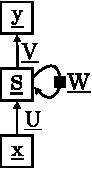
\includegraphics[width=\textwidth]{img/rnn.pdf}}
		\end{minipage}	
		\hspace{0.6cm}
		\begin{minipage}{0.6\textwidth}
		
		\begin{textblock}{10}(5.0,3.5)
			\only<1> {\small define $s_i^{(t)}$ and $y_k^{(t)}$:}
			\only<2> {\small switch from element-wise notation to vector notation}
		\end{textblock}
			\begin{eqnarray*}
			\only<1>{
				s_i^{(t)} &=& \tanh \Big({\smallsum{k=1}{N} U_{ik} \, x_k^{(t)}} 
						{ + \smallsum{j=1}{H}  W_{ij} \, s_j^{(t-1)}}
						+ b^\mathrm{s}_i \Big) \,,
						\\
				y_k^{(t)} &=& f\Big({\smallsum{j=1}{H} 
						V_{kj} \, s_j^{(t)}} + b^\mathrm{y}_k\Big) \,,\\[0.7cm]
					\;\text{e.g.}\;f(\cdot) &:=& \text{e.g. } \mathrm{softmax}(\cdot) \text{ for classification}\\
					}
			\only<2>{
				\vec s^{(t)} &=& \tanh\Big({\vec U \, \vec x^{(t)}} 
						{ + \vec W \, \vec s^{(t-1)}}
						+ \vec b^\mathrm{s} \Big) \,,
						\\
				\vec y^{(t)} &=& f\Big({\vec V \, s^{(t)}} + \vec b^\mathrm{y}\Big) \,,\\[0.7cm]
					\;\text{e.g.}\;f(\cdot) &:=& \text{e.g. } \mathrm{softmax}(\cdot) \text{ for classification}\\
					}
			\end{eqnarray*}
		\end{minipage}
	\end{minipage}
\end{frame}

\subsection{Training RNNs}
\subsubsection{Using the chain rule}

% ------------------------------------------------------------------------------
\begin{frame}\frametitle{\subsecname: \subsubsecname}
	\begin{minipage}{\textwidth} \hspace{5mm}
		\includegraphics<1->[height=4cm]{img/rnn.pdf}
		\hspace{12mm}
		%\includegraphics<2>[height=4cm]{img/rnn_unfolded.pdf}
		%\includegraphics<2>[height=4cm]{img/rnn_unfolded_backprop.pdf}
	\end{minipage}
	\vspace{1mm}
	\begin{itemize}
		\item<1-> cost function $e^{(\alpha,t)}$ for time 
				step $t$ of training sequence $\alpha$ 
			\vspace{-1mm}
			$$
				E^T = \smallfrac{1}{p} \sum\limits_{\alpha=1}^p
				\smallfrac{1}{n_\alpha}\smallsum{t=1}{n_\alpha} e^{(\alpha,t)} \,,
				\quad \text{for training set} \quad 
				\Big\{ \{ \vec x^{(\alpha,t)}, \vec y^{(\alpha,t)} 
					\}_{t=1}^{n_\alpha}\Big\}_{\alpha=1}^{p}
			$$
		\vspace{-1mm}
		\item<2-> gradient computation using the chain rule%by unfolding the network in time 
		\vspace{1mm}
		\item<2-> computational complexity: $\Set O(H^2)$, i.e. quadratic in the number of recurrent weights
		%\item<3-> both $\color{blue}\vec h^{(t)}$ and 
		%		$\color{darkgreen}\vec h^{(t-1)}$ depend on $\vec W$ 
		%		and $\vec U$ ($\leadsto \Set O(n^2)$):
		%	$$
		%		\frac{\partial {\color{blue}h_k^{(t)}}}{\partial W_{ij}}
		%		\quad=\quad 
		%		\Big(f'\big( \vec U \, \vec x^{(t)} 
		%			+ \vec W \, {\color{darkgreen}\vec h^{(t-1)}}
		%			+ \vec b \big) \Big)_k
		%		\cdot \Big( I_{ki} \, {\color{darkgreen}h_j^{(t-1)}} 
		%			+ \smallsum{l}{} W_{kl} 
		%			\smallfrac{\partial {\color{darkgreen}h_l^{(t-1)}}}%
		%				{\partial W_{ij}} \Big)
		%	$$
	\end{itemize}
	\vspace{-2mm}
	\blfootnote{\hfill \citep[for details see][]{Williams95}}
\end{frame}


\subsubsection{Using Backpropagation through time (BPTT)}

% ------------------------------------------------------------------------------
\begin{frame}\frametitle{\subsubsecname}
	\begin{minipage}{\textwidth} \hspace{5mm}
    \mode<presentation>{
		\includegraphics<1->[height=4cm]{img/rnn.pdf}
		\hspace{12mm}
		\includegraphics<1,3>[height=4cm]{img/rnn_unfolded_untie.pdf}
		\includegraphics<2>[height=4cm]{img/rnn_unfolded_bptt.pdf}
        }
    \mode<article>{
		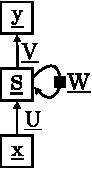
\includegraphics[height=4cm]{img/rnn.pdf}
		\hspace{10mm}
		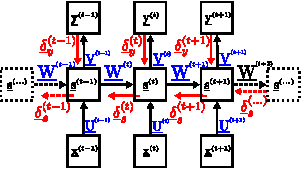
\includegraphics[height=4cm]{img/rnn_unfolded_bptt.pdf}
    }
	\end{minipage}
	\vspace{1mm}
	\begin{itemize}
		\item<1-> assume all unfolded weights, 
				e.g.~$\color{blue}\vec W^{(t)}$, are independent
		\vspace{1mm}
		\item<2-> compute gradients of deep MLP with backpropagation 
				($ \Set O(N)$, where $N$ is the total number of weights)
		\vspace{1mm}
		\item<3-> average all computed gradients, i.e.  
				${\color{blue} \frac{\partial e^{(\alpha,t)}}%
				{\partial \vec W^{(\alpha,\tau)}}}$, 
				for weight update:\\
				\vspace{-1mm}
			$$ \hspace{-5mm}
				\Delta \vec W \;\; = \;\;
					-\eta \, \smallfrac{\partial E^T}{\partial \vec W}
				\;\;=\;\; -\smallfrac{\eta}{p} 
					\smallsum{\alpha=1}{p} \smallfrac{1}{n_{\alpha}}  \smallsum{t=1}{n_{\alpha}}
					\smallfrac{\partial e^{(\alpha, t)}}{\partial \vec W}
				\;\;\approx\;\; -\smallfrac{\eta}{p}
					\smallsum{\alpha=1}{p} \smallfrac{1}{n_{\alpha}} \smallsum{t=1}{n_{\alpha}} \smallfrac{1}{t} \smallsum{\tau=1}{t}
					{\color{blue} \smallfrac{\partial e^{(\alpha,t)}}%
						{\partial \vec W^{(\alpha,\tau)}}}
			$$
	\end{itemize}
\end{frame}

\begin{frame}
\mode<presentation>{
	\begin{minipage}{\textwidth} \hspace{5mm}
		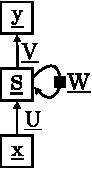
\includegraphics[height=4cm]{img/rnn.pdf}
		\hspace{12mm}
		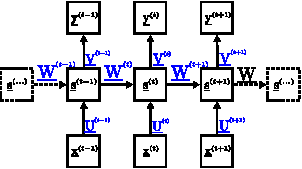
\includegraphics[height=4cm]{img/rnn_unfolded_untie.pdf}
	\end{minipage}
	\vspace{1mm}
	\begin{itemize}
		\item[]
			$$ \hspace{-5mm}
				\Delta \vec W
				\;\;\approx\;\; -\smallfrac{\eta}{p}
					\smallsum{\alpha=1}{p} \smallfrac{1}{n_{\alpha}} \smallsum{t=1}{n_{\alpha}} \smallfrac{1}{t} \smallsum{\tau=1}{t}
					{\color{blue} \smallfrac{\partial e^{(\alpha,t)}}%
						{\partial \vec W^{(\alpha,\tau)}}}
			$$
	\end{itemize}
	}
The backpropagation algorithm provides an \emph{exact} computation of the gradients.
However, 
since BPPT involves unfolding the weights (unrolling the network), this leads to an \emph{approximation of the gradients}.
\end{frame}

\mode*

\clearpage

\mode<all>
\section{Vanishing and exploding of gradients}

\definecolor{darkgreen}{rgb}{0,0.5,0}
\definecolor{darkyellow}{rgb}{0.5,0.5,0}
\definecolor{midgreen}{rgb}{0,0.75,0}


\begin{frame}\frametitle{Motivation}
	\begin{itemize}
	\setlength\itemsep{1cm}
	\item[]
	A simple RNN learns from short-term errors faster (exponentially)\\
	than from errors due to longer ($\Delta t >\!\!> 1$) distances in a sequence.\\
	
	\item[]Example:\\Estimating the topic of a lengthy text where the ``clue'' is mentioned in the very beginning.\\
	
	\item[]The gradient vanishes.
	\end{itemize}
\end{frame}

\subsection{The Vanishing Gradient Problem leads to exponential forgetting}

\begin{frame}\frametitle{A simple RNN}
	\begin{minipage}{\textwidth}
		\begin{minipage}{0.21\textwidth}
        \mode<presentation>{
			{\includegraphics<1>[width=\textwidth]{img/rnn.pdf}}
            }
			{\includegraphics<2>[width=\textwidth]{img/rnn_superscript.pdf}}
		\end{minipage}	
		\hspace{0.6cm}
		\begin{minipage}{0.6\textwidth}
		
		\begin{textblock}{10}(5.0,3.5)
			\only<2> {\small add superscripts to the different weight matrices}
		\end{textblock}
			\begin{eqnarray*}
             \slidesonly{  
			\only<1>{
				\vec s^{(t)} &=& \tanh\Big({\vec U \, \vec x^{(t)}} 
						{ + \vec W \, \vec s^{(t-1)}}
						+ \vec b^\mathrm{s} \Big) \,,
						\\
				\vec y^{(t)} &=& f\Big({\vec V \, s^{(t)}} + \vec b^\mathrm{y}\Big) \,,\\[0.7cm]
					\;\text{e.g.}\;f(\cdot) &:=& \text{e.g. } \mathrm{softmax}(\cdot) \text{ for classification}\\
					}
                    }
			\only<2>{
				\vec s^{(t)} &=& \tanh\Big({\vec U^\mathrm{h} \, \vec x^{(t)}} 
						{ + \vec W^\mathrm{h} \, \vec s^{(t-1)}}
						+ \vec b^\mathrm{s} \Big) \,,
						\\
				\vec y^{(t)} &=& f\Big({\vec V^\mathrm{y} \, \vec s^{(t)}} + \vec b^\mathrm{y}\Big) \,,\\[0.7cm]
					\;\text{e.g.}\;f(\cdot) &:=& \text{e.g. } \mathrm{softmax}(\cdot) \text{ for classification}\\
					}
			\end{eqnarray*}
		\end{minipage}
	\end{minipage}
\end{frame}

% ------------------------------------------------------------------------------
\begin{frame}\frametitle{Exponential forgetting}
	\iitem{an RNN with no inputs and a linear transfer function}
	\vspace{1mm}
	$$
		\vec s^{(t)} 
		\quad = \quad \vec W \, \vec s^{(t-1)}
		\quad=\quad (\vec W)^t \, \vec s^{(0)}
	$$
	\pause
	\iitem{eigenvalue decomposition:
		$\vec W = \vec U \, \vec \Lambda \, \vec U^\top$}
	\vspace{1mm}
	$$
		\vec s^{(t)} \quad =\quad 
			\underbrace{\vec U
			}_{\kern-3ex\text{\footnotesize rotate back}\kern-3ex}
			\overbrace{(\vec \Lambda)^t
			}^{\kern-6ex\text{\footnotesize exponential scaling}\kern-6ex}
			\underbrace{\vec U^\top \vec s^{(0)}
			}_{\text{\footnotesize rotation}}
	$$
	\pause
	\iitem{long-term activity dominated by the largest $|\lambda_{1}|$ 
		%grows fastest / shrinks slowest
		\vspace{1mm}
		\iitem{$|\lambda_{1}| > 1 \quad 
			\leadsto \quad \lim\limits_{t\to\infty} s_i^{(t)} = \pm \infty\,,
				\forall i$
			\hfill (exploding activity)}
		\vspace{-2mm}
		\iitem{$|\lambda_{1}| < 1 \quad 
			\leadsto \quad \lim\limits_{t\to\infty} s_i^{(t)} = 0 \,,
				\forall i$
			\hfill (vanishing activity)}
	}
	%\blfootnote{\hfill\citep[Section 10.7]{Goodfellow16}}
\end{frame}

% ------------------------------------------------------------------------------
\begin{frame}\frametitle{Vanishing gradients}
\mode<presentation>{
	\begin{minipage}{\textwidth} \hspace{5mm}
		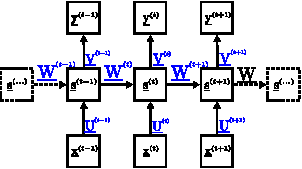
\includegraphics[height=4cm]{img/rnn_unfolded_untie.pdf}
	\end{minipage}
	}
	%~ \iitem{local error terms $\vec \delta^{(t)}$ in backpropagation through time
	\iitem{local error terms in backpropagation through time
		\vspace{1mm}
		%\iitem{for transfer function $f(h) = \tanh(h)$, 
				%i.e.~$f'(h) = \big(1 - f^2(h)\big)$\\
				%%~ and total input $z_i^{(t)} = \smallsum{j=1}{H} W_{ij} h_j^{(t-1)}$
                %}
				}
	%~ \vspace{2mm}
	%$$
		%\delta_i^{(t)} 
		%%quad=\quad \smallfrac{\partial E^T}{\partial h_i^{(t)}}
		%\quad=\quad \smallfrac{\partial y^{(t)}}{\partial z_i^{(t)}}
		%%\quad=\quad \Big(\kern-1.5ex\underbrace{1 - \big(h_i^{(t)}\big)^2
		%\quad=\quad \Big(\kern-1.5ex\underbrace{1 - f^2\big(z_i^{(t)}\big)
				%}_{\begin{array}{c}\\[-4mm]
					%\text{\scriptsize derivative < 1} \\[-1.5mm]
					%\text{\scriptsize i.e.~contracting} 
				%\end{array}} \kern-1.5ex\Big)
			%\cdot \Big(\underbrace{\smallsum{j=1}{H} W_{ij}^\top \delta_j^{(t+1)}
				%}_{\kern-2ex\begin{array}{c}\\[-6mm]
					%\text{\scriptsize potentially} \\[-1.75mm]
					%\text{\scriptsize exploding/vanishing}
				%\end{array}\kern-2ex}\Big)
	%$$
	%~ \vspace{2mm}
	%~ \iitem{over many time steps the local errors $\delta_i^{(t)}$ often vanish}
	\iitem{over many time steps the local errors may also vanish}
		%\vspace{1mm}
		%\iitem{large $\vec w_i \Rightarrow h_i^{(t)} \approx 1 \Rightarrow$ 
		%	derivative $\approx 0$}
		%\iitem{rarely explodes thanks to anti-cyclical derivative $<1$}
	\vspace{2mm}
	\iitem{small short-term errors overshadow large long-term errors}
	%\vspace{2mm}
	%\begin{center}\bf 
	%	How can we learn long time-series without vanishing gradients?
	%\end{center}
\end{frame}


\mode*

\clearpage

\mode<all>
\section{Echo-state networks}

\definecolor{darkgreen}{rgb}{0,0.5,0}
\definecolor{darkyellow}{rgb}{0.5,0.5,0}
\definecolor{midgreen}{rgb}{0,0.75,0}

% ------------------------------------------------------------------------------
\begin{frame}\frametitle{Echo-state networks}
	\placeimage{13.75}{0.75}{img/rnn.pdf}{height=3cm}
		\iitem{system dynamics determine the input representation
			\vspace{1mm}
			\iitem{non-linear preprocessing step with memory}}
		\vspace{4mm}
		\iitem{address vanishing gradients by keeping $\vec W$ and $\vec U$ fixed
			\vspace{1mm}
			\iitem{output weights $\vec V$ can be trained by e.g.~linear regression}
			\vspace{-1mm}
			\iitem{hidden ``reservoir'' maintains inputs/errors over time}
			%\vspace{-2mm}
			%\iitem{hidden dynamics must be rich enough to bridge the gap}
		}
		\vspace{4mm}
		\iitem{system dynamics determine how fast inputs/errors are forgotten}
	\blfootnote{\hfill\citep[Section 10.8]{Jaeger04,Goodfellow16}}
\end{frame}

\subsection{Initialization of weight matrices}

% ------------------------------------------------------------------------------
\begin{frame}\frametitle{Echo-state networks: Careful weight initialization}
	\placeimage{13.75}{0.75}{img/rnn.pdf}{height=3cm}
		\iitem{eigenvalues $\lambda_i$ of the system's {\em Jacobian} $\vec J$}
			$$
				J_{ij}^{(t)} 
				\quad=\quad 
				%~ \smallfrac{\partial h_i^{(t)}}{\partial h_j^{(t-1)}}
				%~ \quad=\quad
				%~ f'\big(h_i^{(t)}\big) \cdot W_{ij}
				\smallfrac{\partial h_i^{(t)}}{\partial h_j^{(t-1)}}
				\quad=\quad
				 W_{ij} \, f'\big(h_j^{(t)}\big)
				\hspace{2cm}
			$$
            $$
                h_i^{(t)} = \smallsum{j=1}{H} W_{ij} \, f(h_j^{(t-1)})
            $$
		\vspace{2mm}
		\iitem{eigenvectors with $|\lambda_i| \approx 1$ 
				vanish/explode {\em very slowly}
			\vspace{1mm}
			\iitem{inputs/errors are maintained for a long time}}
		\vspace{6mm}
		\iitem{generate random $\vec W$, and $\vec U$ 
				where all $|\lambda_j| \approx r$
			\vspace{1mm}
			%~ \iitem{$f'(h_i^{(t)}) < 1$ \quad is a contraction $\quad\leadsto\quad$ $r > 1$}
			\iitem{$f'(h_j^{(t)}) < 1$ \quad is a contraction $\quad\leadsto\quad$ $r > 1$}
			\vspace{-1mm}
			\iitem{values between $r=1.2$ and $r=3$ are used in practice}
			\vspace{-2mm}
			%\iitem{$n$ hidden neurons can maintain
					%inputs/errors for up to $n$ time steps }
					}
	\blfootnote{\hfill\citep[Section 10.8]{Jaeger04,Goodfellow16}}
\end{frame}


\mode*

\clearpage

\mode<all>
\section{From RNN to LSTM}

\definecolor{darkgreen}{rgb}{0,0.5,0}
\definecolor{darkyellow}{rgb}{0.5,0.5,0}
\definecolor{midgreen}{rgb}{0,0.75,0}

\begin{frame}\frametitle{What is an LSTM?}
The long short-term memory (LSTM) cell is an extension of the basic RNN
architecture with memory cells.
\end{frame}

% ------------------------------------------------------------------------------
\begin{frame}\frametitle{Long short-term memory (LSTM) architecture}
    \mode<presentation>{
	\begin{textblock}{}(10.25,2.5)
		%\includegraphics<1>[height=3cm]{img/lstm_feedback.pdf}
		\includegraphics<1>[height=3cm]{img/lstm_feedback_delay.pdf}
		%\includegraphics<2>[height=3cm]{img/lstm_write.pdf}
		\includegraphics<2>[height=3cm]{img/lstm_write_delay.pdf}
		%\includegraphics<3->[height=3cm]{img/lstm.pdf}
		\includegraphics<3->[height=3cm]{img/lstm_delay_indices.pdf}
	\end{textblock}
    }
    \mode<article>{
	\begin{textblock}{}(10.25,2.5)
		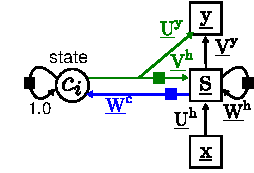
\includegraphics[height=3cm]{img/lstm_feedback_delay.pdf}\\
        
		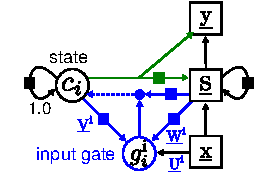
\includegraphics[height=3cm]{img/lstm_write_delay.pdf}\\
        
		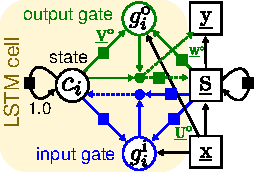
\includegraphics[height=3cm]{img/lstm_delay_indices.pdf}
	\end{textblock}
    }
	
	\begin{textblock}{10}(0.4,2.5)
		\only<1>{ \small
			\iitem{extend the simple RNN with state nodes $\vec s$}
			\vspace{-5mm}
			\iitem{leaky unit $s_i$ with $\alpha_i=1$}
			\vspace{-5mm}
			\iitem{{\color{darkgreen}time delayed feedback} to hidden layer}
			\vspace{-5mm}
			\iitem{{\color{blue} transfer function} 
					$\sigma(x) = \big( 1 + e^{-x} \big)^{-1}$
					}
		} \only<2>{ \small
			\iitem{introducing an {\color{blue}input (``write'') gate 
					$g_i^\mathrm{i}$}
					\vspace{-2mm}
					\iitem{\footnotesize gate transfer function
							$\sigma(x) = \big( 1 + e^{-x} \big)^{-1}$} }
			\vspace{-4mm}
			\iitem{state input is multiplied ($\color{blue}\otimes$) with gate}
			\vspace{-5mm}
			\iitem{state $s_i$ only changes when 
					{\color{blue}$g_i^{\mathrm{i}(t)} \gg 0$}}
			\vspace{-5mm}
			\iitem{local errors $\delta_i^{(t)}$ still accumulate in $s_i$}
		} \only<3>{ \small
			\iitem{introducing an {\color{darkgreen}output 
					(``read'') gate $g_i^\mathrm{o}$}
					\vspace{-2mm}
					\iitem{\footnotesize gate transfer function
							$\sigma(x) = \big( 1 + e^{-x} \big)^{-1}$} }
			\vspace{-4mm}
			\iitem{state output is multiplied 
					($\color{darkgreen}\otimes$) with gate}
			\vspace{-5mm}
			\iitem{error $\delta_i^{(t)}$ only changes when 
					{\color{darkgreen}$g_i^{\mathrm{o}(t)} \gg 0$}}
			\vspace{-4mm}
			\iitem{both gates and the state form a {\color{darkyellow}LSTM cell}}
		} \only<4>{ \small\vspace{-1mm}
			\iitem{gates determine access to the state $s_i$
				\vspace{-1mm}
				\iitem{$\color{blue}g_i^{\mathrm{i}}$  learns 
					what to remember}
				\vspace{-3mm}
				\iitem{$\color{darkgreen}g_i^\mathrm{o}$ 
					learns when use the memory} }
			\vspace{-4mm}
			\iitem{gates regulate the flow of activity and error
				\vspace{-1mm}
				\iitem{$\color{blue}g_i^{\mathrm{i}}$ regulates 
						the forward-pass}
				\vspace{-3mm}
				\iitem{$\color{darkgreen}g_i^\mathrm{o}$ 
					regulates the backward-pass} }
		}
	\end{textblock}
	
	\begin{textblock}{10}(0.8,7.5)
	\small
	\begin{eqnarray*}
		\vec c^{(t)} &=& \vec  c^{(t-1)} 
				+  {\color{blue} \visible<2->{ \vec g^{\mathrm{i}(t)} \odot}  \tanh\Big( 
					\vec W^\mathrm{c} \vec s^{(t-1)} \Big)
					 } \\[-1mm]
		\vec y^{(t)} &=& f\Big( \vec V^\mathrm{y} \, \vec s^{(t)} + \vec b^\mathrm{y}
					+ {\color{darkgreen} \vec U^\mathrm{y} 
					\visible<3->{\big(} \vec c^{(t)} 
					\visible<3->{\odot \vec g^{\mathrm{o}(t)} \big)} } 
					\Big) \,,
					\qquad \text{e.g.}\;f(\cdot)=\text{softmax}(\cdot) \\[-1mm]
		\vec s^{(t)} &=& \tanh\Big( \vec U^\mathrm{h} \, \vec x^{(t)}  
				+ \vec W^\mathrm{h} \, \vec s^{(t-1)} + \vec b^\mathrm{s}
				+ {\color{darkgreen} \vec V^\mathrm{h} 
					\visible<3->{\big(} \vec c^{(t-1)} 
					\visible<3->{\odot \vec g^{\mathrm{o}(t)} \big)} }
				\Big) \\[-1mm]
		\visible<2->{\color{blue} \vec g^{\mathrm{i}(t)}} 
			&\visible<2->{\color{blue}=}& 
			\visible<2->{\color{blue}
				\sigma\Big(\vec U^\mathrm{i} \, \vec x^{(t)} 
				+ \vec V^\mathrm{i} \, \vec c^{(t-1)} 
				+ \vec W^\mathrm{i} \, \vec s^{(t-1)} 
				+ \vec b^\mathrm{i} \Big) } \\[-1mm]
		\visible<3->{\color{darkgreen} \vec g^{\mathrm{o}(t)}} 
			&\visible<3->{\color{darkgreen}=}& 
			\visible<3->{\color{darkgreen}
				\sigma\Big(\vec U^\mathrm{o} \, \vec x^{(t)} 
				+ \vec V^\mathrm{o} \, \vec c^{(t-1)} 
				+ \vec W^\mathrm{o} \, \vec s^{(t-1)} 
				+ \vec b^\mathrm{o} \Big) } 
	\end{eqnarray*}	
	
	
	\only<4>{
	\vspace{-5mm}
	
	\question{Why does ${\color{blue}\tanh(\cdot)}$ make sense here?
	}
	}
	
	\end{textblock}
	
	
	\begin{textblock}{20}(2.75,14.9)
		\footnotesize\only<1-2>{\citep[Section 10.10]{Hochreiter97,Goodfellow16}}
	\end{textblock}
	
	
\end{frame}

\newpage

\begin{frame}\frametitle{LSTM with forget gate}
\begin{figure}[ht]
     \centering
	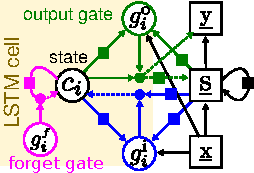
\includegraphics[width=0.4\textwidth]{img/lstm_delay_forget.pdf}
     \mode<article>{
	\caption{Basic RNN architecture}
	}
	\label{fig:rnn} 
\end{figure}
\pause

\begin{equation}
		{\color{magenta} \vec g_i^{\mathrm{f}(t)}} 
			= 
			\color{magenta}
				\sigma\Big(\vec U^\mathrm{f} \, \vec x^{(t)} 
				+ \vec V^\mathrm{f} \, \vec c^{(t-1)} 
				+ \vec W^\mathrm{f} \, \vec s^{(t-1)} 
				+ \vec b^\mathrm{f} \Big) 
\end{equation}

Consequently:
\begin{equation}
		\vec c^{(t)} = {\color{magenta}\vec g^{\mathrm{f}(t)} \odot\,} \vec  c^{(t-1)} 
				+  {\color{blue} { \vec g^{\mathrm{i}(t)} \odot}  \tanh\Big( 
					\vec W^\mathrm{c} \vec s^{(t-1)} \Big)
					 }
\end{equation}


\end{frame}

\begin{frame}\frametitle{Complexity}
\mode<presentation>{
\only<1>{
			\placeimage{13}{1}{img/rnn_superscript}{width=2cm}
			}
\only<2->{
			\placeimage{9}{1}{img/lstm_delay_forget}{width=5cm}
			}
}
		For $\vec x \in \R^N, \vec s \in \R^H, \vec y \in \R^M$:\\
		\begin{itemize}
		\item[]
			Simple RNN:\\
			\begin{itemize}
			\item $\vec U^{\mathrm{h}} \in \R^{H,N},\quad \vec b^{\mathrm{h}} \in \R^{H}$
			\item $\vec W^{\mathrm{h}} \in \R^{H,H}$
			\item $\vec V^{\mathrm{y}} \in \R^{M,H},\quad \vec b^{\mathrm{y}} \in \R^{M}$
			\end{itemize}
			\pause
			
		\item[]
			LSTM:\\
			All of the above in addition to\ldots
			for $\vec c, {\color{blue}\vec g^{\mathrm{i}}}, {\color{darkgreen}\vec g^{\mathrm{o}}}, {\color{magenta}\vec g^{\mathrm{f}}} \in \R^K$\\
			(often $K=H$):\\
			\pause
			\begin{itemize}
			\item for $\vec c$:
             $\color{blue}\vec W^{\mathrm{c}} \in \R^{K,H}$, 
			 $\color{darkgreen}\vec U^{\mathrm{y}} \in \R^{M,K}$,
			 $\color{darkgreen}\vec V^{\mathrm{h}} \in \R^{H,K}$
			\item[] for ${\color{blue}\vec g^{\mathrm{i}}}$:
            \begin{itemize}
                \item $\color{blue}\vec U^{\mathrm{i}} \in \R^{K,N}$
                \item $\color{blue}\vec V^{\mathrm{i}} \in \R^{K,K}$
                \item $\color{blue}\vec W^{\mathrm{i}} \in \R^{K,H}, \quad \vec b^{\mathrm{i}} \in \R^{K}$
			\end{itemize}
            \item duplicate $\color{blue}\vec U^{\mathrm{i}}, \color{blue}\vec V^{\mathrm{i}}, \color{blue}\vec W^{\mathrm{i}}$
			for the output gate $\leadsto \color{darkgreen}\vec U^{\mathrm{o}}, \color{darkgreen}\vec V^{\mathrm{o}}, \color{darkgreen}\vec W^{\mathrm{o}}$ and $\color{darkgreen}\vec b^{\mathrm{o}}$
			\item and for the forget gate $\leadsto \color{magenta}\vec U^{\mathrm{f}}, \color{magenta}\vec V^{\mathrm{f}}, \color{magenta}\vec W^{\mathrm{f}}$ and $\color{magenta}\vec b^{\mathrm{f}}$
			\end{itemize}
		\end{itemize}
        
        \pause
		\question{What about the complexity of echo state networks?}

\mode<article>{
        - The hidden-output weights $\vec V$ are the only trainable parameters in echo state networks.
}
\end{frame}

\mode*

\clearpage

%\mode<all>
%\mode<presentation>{

\begin{frame}\frametitle{Unrolling the LSTM in time (the build up - memory states)}
	An alternative visualization of the LSTM cell without delay blocks. We can unroll the network in time to see how the units interact with one another.

	\begin{center}
	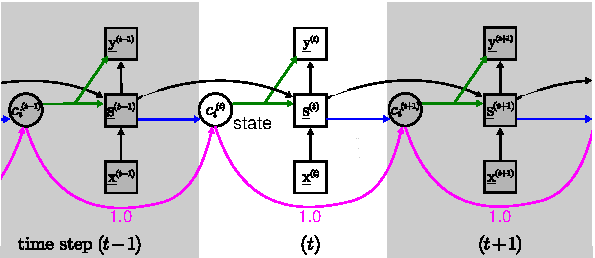
\includegraphics[width=0.9\textwidth]{img/lstm_delay_unroll_memory}
	\captionof*{figure}{Connecting states to hidden \& output units}
	\end{center}
\end{frame}

\begin{frame}\frametitle{Unrolling the LSTM in time (the build up - writing to memory)}
	\begin{center}
	\only<1>{
	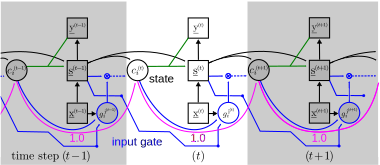
\includegraphics[width=0.9\textwidth]{img/lstm_delay_unroll_write_connect_bubbles}
	\captionof*{figure}{Adding input gates for writing}
	}
	\only<2>{
	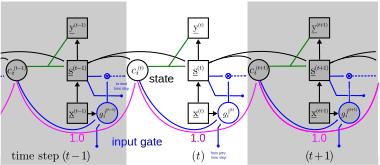
\includegraphics[width=0.9\textwidth]{img/lstm_delay_unroll_write}
	\captionof*{figure}{Adding input gates for writing (keep connections but reduce clutter)}
	}
	\end{center}
\end{frame}
}

\begin{frame}\frametitle{
Unrolling the LSTM in time
(the build up - reading from memory)
}

\mode<article>{
\underline{Unrolling the LSTM in time}:\\

An alternative visualization of the LSTM cell without delay blocks. We can unroll the network in time to see how the units interact with one another.
}

\mode<presentation>{
\placeimage{11.7}{2.2}{img/lstm_delay_indices}{width=33mm}
\vspace{22mm}
}

\begin{figure}[h]
	\centering
	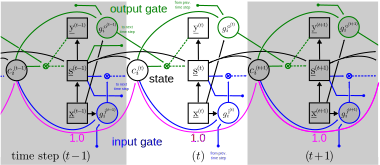
\includegraphics[width=0.9\textwidth]{img/lstm_delay_unroll}
	\mode<article>{
	\caption{Unrolling the LSTM cell with input and output gates in time.}
	}
	\mode<presentation>{
	\captionof*{figure}{Adding output gates for reading}
	}
\end{figure}

\end{frame}

%\mode*

%\clearpage

\end{rightcolumn}
\end{paracol}

\end{document}
